\documentclass{article}

\usepackage{enumerate}
\usepackage{amssymb}
\usepackage{amsmath}
\usepackage{algorithm}
\usepackage{physics}
\usepackage{listings}
\usepackage[noend]{algpseudocode}
\usepackage{graphicx}

\graphicspath{ {./} }

\topmargin=-0.45in
\evensidemargin=0in
\oddsidemargin=0in
\textwidth=6.5in
\textheight=9.0in
\headsep=0.25in

\title{Chem 195: Problem Set 8}
\author{Michael Stephen Chen}


\begin{document}
\maketitle
\pagebreak

\section*{Problem 1}
\begin{enumerate}[i.]
  \item See \textit{randint.m}.
  \item See \textit{histo\_int.data}
  \item When sampling integers ($N_{samp}=15000$) between 1 and 10 using \textit{randint.m}, I get the following normalized distribution.
    \begin{center}
      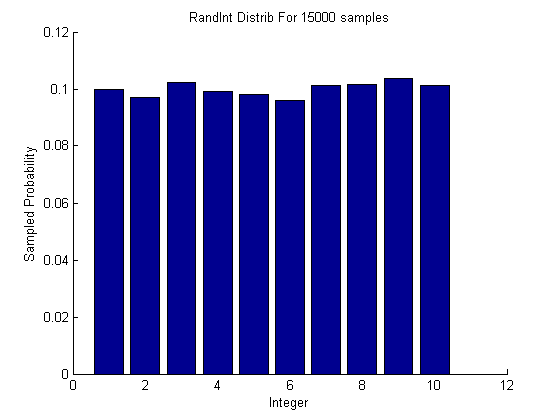
\includegraphics[scale=0.5]{prob1part3}
    \end{center}
  \item We use equation (1) to estimate the order of the error in our esimate of $p(n) = 0.1$. We do this for $N_{samp}=100, 10000, 1000000$.
    \begin{center}
      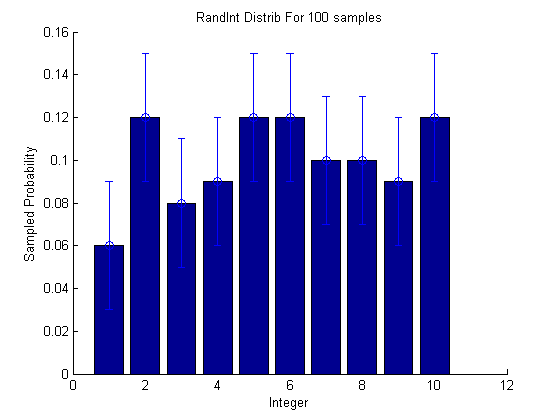
\includegraphics[scale=0.5]{prob1part4_1}

      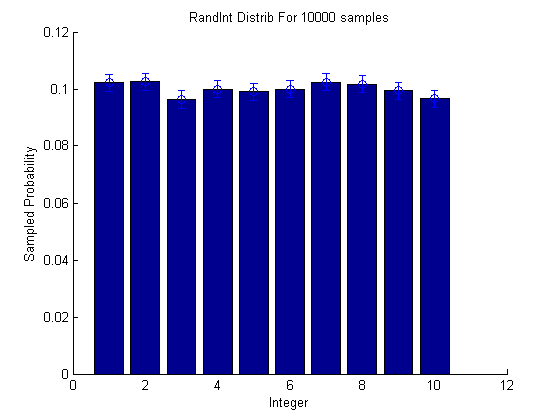
\includegraphics[scale=0.5]{prob1part4_2}

      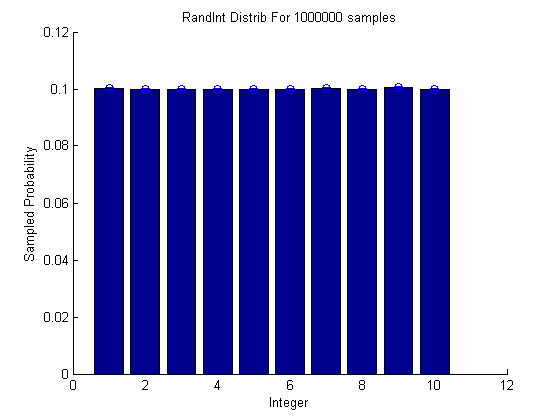
\includegraphics[scale=0.5]{prob1part4_3}
    \end{center}
    For each of these trials, we see that indeed the sampled probabilities for all the integers deviate as expected from the actual probability of $p(n) = 0.1$.
\end{enumerate}

\section*{Problem 2}
\begin{enumerate}[i.]
  \item See \textit{ho.m}
  \item The following MC simulation was run with $M=10$ and $E=50$. A black line is drawn at the expectation value $n_i=5$.
    \begin{center}
      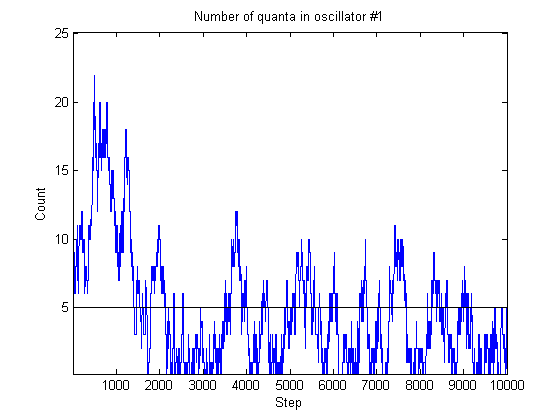
\includegraphics[scale=0.5]{prob2part2}
    \end{center}
    Qualitatively we estimate the typical ``time'' of deviation (the number of steps) from the expectation to be on the order of $\tau=100$.
  \item The following MC simulation was run with $M=100$ and $E=500$. A black line is drawn at the expectation value $n_i=5$.
    \begin{center}
      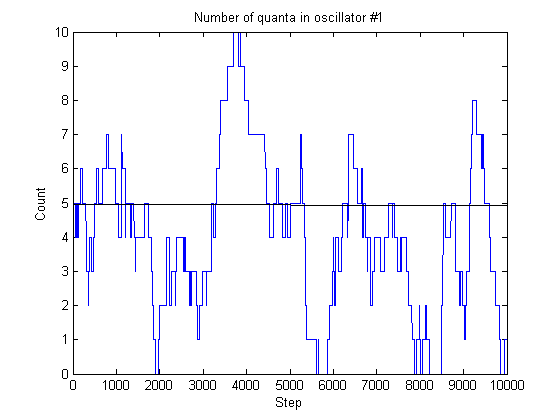
\includegraphics[scale=0.5]{prob2part3}
    \end{center}
    Qualitatively we estimate the typical ``time'' of deviation (the number of steps) from the expectation to be on the order of $\tau=1000$.

    It makes sense to report results in terms of the total number of steps ($N_{steps}$) per degree of freedom ($M$), or sweeps, because as we see in parts (ii) and (iii) the deviations from the expectation are longer when we have more degrees of freedom. This is because at each step, our simulation chooses two oscillators at random to exchange quanta. When there are more oscillators, the probability of choosing any one oscillator is less ($1/M$) so it takes more steps on average to ``touch'' any single oscillator. To normalize for this, we report in sweeps.

  \item Qualitatively, we can associate the $\tau$ from parts (ii) and (iii) as the number of steps required on average for one independent sample of $n_1$. This is because we assume that by the time $n_1$ returns to its expectation value it has essentially returned to ``square one'', or its initial ``memoryless'' state; the value of $n_i$ is highly correlated from one step to the other since there is a high probabilty that $n_i$ at step $n$ will equal $n_i$ at step $n+1$.
    So using our estimates from (ii) and (iii), we estimate that the number of steps on average for one independent sample is 100 and 1000 respectively. This equates to 10 and 10 sweeps, respectively. So for both, the number of independent samples is $10t$, where $t$ is the number of sweeps.

  \item For $M=30$, $E=30$, and $N^*_{step}=100000$ we get the following histogram. Note that $p(n=1)=0.254$ and that at every $N^*_{step}$  we consolidate the statistics for all $M$ of the oscillators.
    \begin{center}
      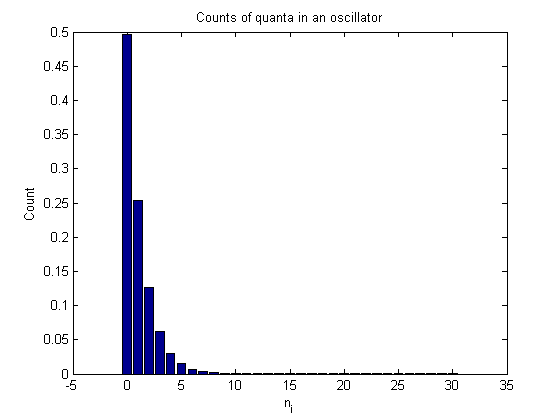
\includegraphics[scale=0.5]{prob2part5}
    \end{center}

  \item To determine the expected probabilty of $p(n=1)$, we observe that this is essentially a ``stars and bars'' problem. When there are $n$ balls and $k$ bins, the total number of configurations is given by:
    $$\binom{n+k-1}{n}$$

  Let us find the probability that one specific oscillator has one quanta. This probability is given by the proportion of configurations that have that one oscillator fixed with one quanta:
  $$p(n_i=1) = \frac{\binom{30+30-1}{30}}{\binom{29+29-1}{29}} = 0.25424$$

  After running the simulaton 10 times, I found that the average number of steps $N^*_{steps}$ for $p(n=1)$ to converge within $\epsilon = 0.01$ was $6530.4$.

  \item We keep in mind that each $N^*_{step}$ is essentiall one sweep. From our predictions in the previous problems, we esimated the number of independent samples to be $10t$, where $t$ is the number of sweeps. So based on that, we would estimate that the number of indpendent samples that go into our estimte for part (vi) to be
    $$10N^*_{steps} = 10 \times 6530.4 = 65304$$

  \item We expect that $p(n)$ decays with increasing $n$, and we can expain this combinatorially. Since all allowed microstates have equal probability, the probability of a certain configuration is ratio of the number of that configuration over the total number of possible configurations. Again we can think in terms of ``stars and bars'' or ``balls and bins'' like in part(vi). Thus when any one oscillator (bin) has more quanta (balls), that means that there are less balls to distribute amongst the other bins. So as we increase the amount of balls in one bin, the number of such configurations goes down and hence the probability goes down as well.

  \item The decay of $p(n)$ does indeed appear to be exponential. There is a very good linear fit for low values of $n$. For higher values, the small counts are inherently susceptible to random fluctuations so deviations from linearity are expected.
    \begin{center}
      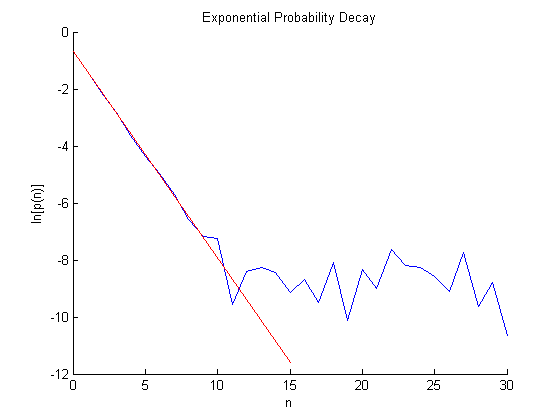
\includegraphics[scale=0.5]{prob2part9}
    \end{center}
    The red line above has a slope $\beta = 0.7291$ and an intercept of $\alpha = -0.6596$.

  \item Below is a scatter plot plotting $\bar{n}$ vs. $1/\beta$ for $E = 1, 2,..., 30$, where $\bar{n} = E / M$ and $\beta$ is defined as in part (ix).
    \begin{center}
      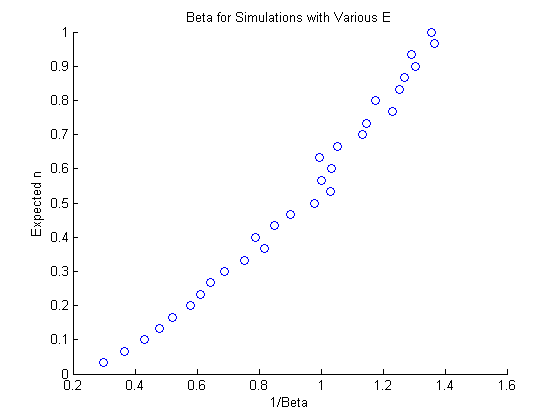
\includegraphics[scale=0.5]{prob2part10}
    \end{center}
    
    Below is a table comparing our results with the known values. Note that are all roughly within $0.1$.
    \begin{center}
      $\begin{array}{c|c|c|c}
        \beta & \bar{n}_{sim} & \bar{n}_{known} & Error \\ \hline
        3.367 & 0.033 & 0.036 & 0.067 \\ 
        2.738 & 0.067 & 0.069 & 0.036 \\ 
        2.322 & 0.100 & 0.109 & 0.080 \\ 
        2.085 & 0.133 & 0.142 & 0.060 \\ 
        1.922 & 0.167 & 0.171 & 0.028 \\ 
        1.726 & 0.200 & 0.217 & 0.077 \\ 
        1.632 & 0.233 & 0.243 & 0.040 \\ 
        1.557 & 0.267 & 0.267 & 0.002 \\ 
        1.451 & 0.300 & 0.306 & 0.020 \\ 
        1.326 & 0.333 & 0.362 & 0.078 \\ 
        1.223 & 0.367 & 0.417 & 0.121 \\ 
        1.267 & 0.400 & 0.392 & 0.020 \\ 
        1.177 & 0.433 & 0.445 & 0.027 \\ 
        1.107 & 0.467 & 0.494 & 0.054 \\ 
        1.022 & 0.500 & 0.562 & 0.111 \\ 
        0.972 & 0.533 & 0.609 & 0.124 \\ 
        0.999 & 0.567 & 0.582 & 0.027 \\ 
        0.967 & 0.600 & 0.613 & 0.022 \\ 
        1.004 & 0.633 & 0.579 & 0.095 \\ 
        0.949 & 0.667 & 0.632 & 0.055 \\ 
        0.882 & 0.700 & 0.706 & 0.009 \\ 
        0.871 & 0.733 & 0.719 & 0.019 \\ 
        0.813 & 0.767 & 0.797 & 0.039 \\ 
        0.851 & 0.800 & 0.745 & 0.074 \\ 
        0.799 & 0.833 & 0.818 & 0.019 \\ 
        0.788 & 0.867 & 0.835 & 0.038 \\ 
        0.767 & 0.900 & 0.867 & 0.038 \\ 
        0.774 & 0.933 & 0.855 & 0.091 \\ 
        0.732 & 0.967 & 0.927 & 0.043 \\ 
        0.737 & 1.000 & 0.917 & 0.090 \\ 
      \end{array}$
    \end{center}
\end{enumerate}

\end{document}
